\documentclass[12pt]{../manual}
%____________________________________________________________________________
%
%	TITLE AND TABLE OF CONTENTS
%____________________________________________________________________________
\begin{document}
\makeheader{Mask Design}
\begin{center}
\textbf{\huge ECE 230L}\\~\\
\textbf{\large MASK DESIGN INSTRUCTIONS}\\~\\
\rule{6.5in}{0.5mm}\\
\end{center}
%____________________________________________________________________________
%
%	BODY
%____________________________________________________________________________
\section{Creating your workspace}
\begin{enumerate}
\item Go to \url{duke.onshape.com} and sign in
\item Select the {\bf Documents} tab on the top left and then click {\bf Create} $\to$ {\bf Document}
\begin{figure}[ht!]
\centering
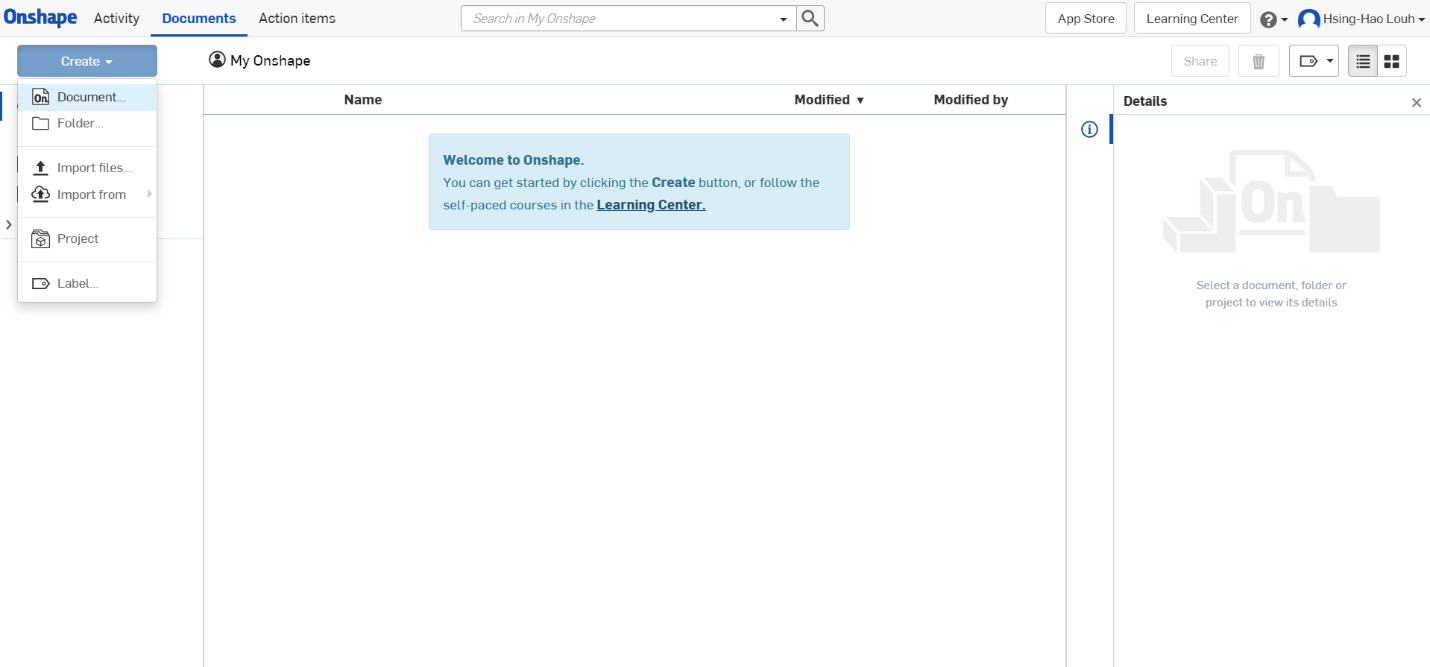
\includegraphics[width=0.8\textwidth]{figures/image1.png}
\caption{Documents tab and dropdown menu}
\end{figure}
\item Click on the menu button $\vcenter{\hbox{
\includegraphics{figures/image2.png}}}$ on the top left and select {\bf Workspace units}. Change the {\bf Default length unit} to Millimeter.
\end{enumerate}
\newpage
\section{Creating your mask}
\begin{enumerate}
\setcounter{enumi}{3}
\item On the cube in the top right, click on the surface that says {\bf Top}. This is the plane we will be working on. Right click on the Top plane and select {\bf Hide other planes}. Your screen should look like this:
\begin{figure}[ht!]
\centering
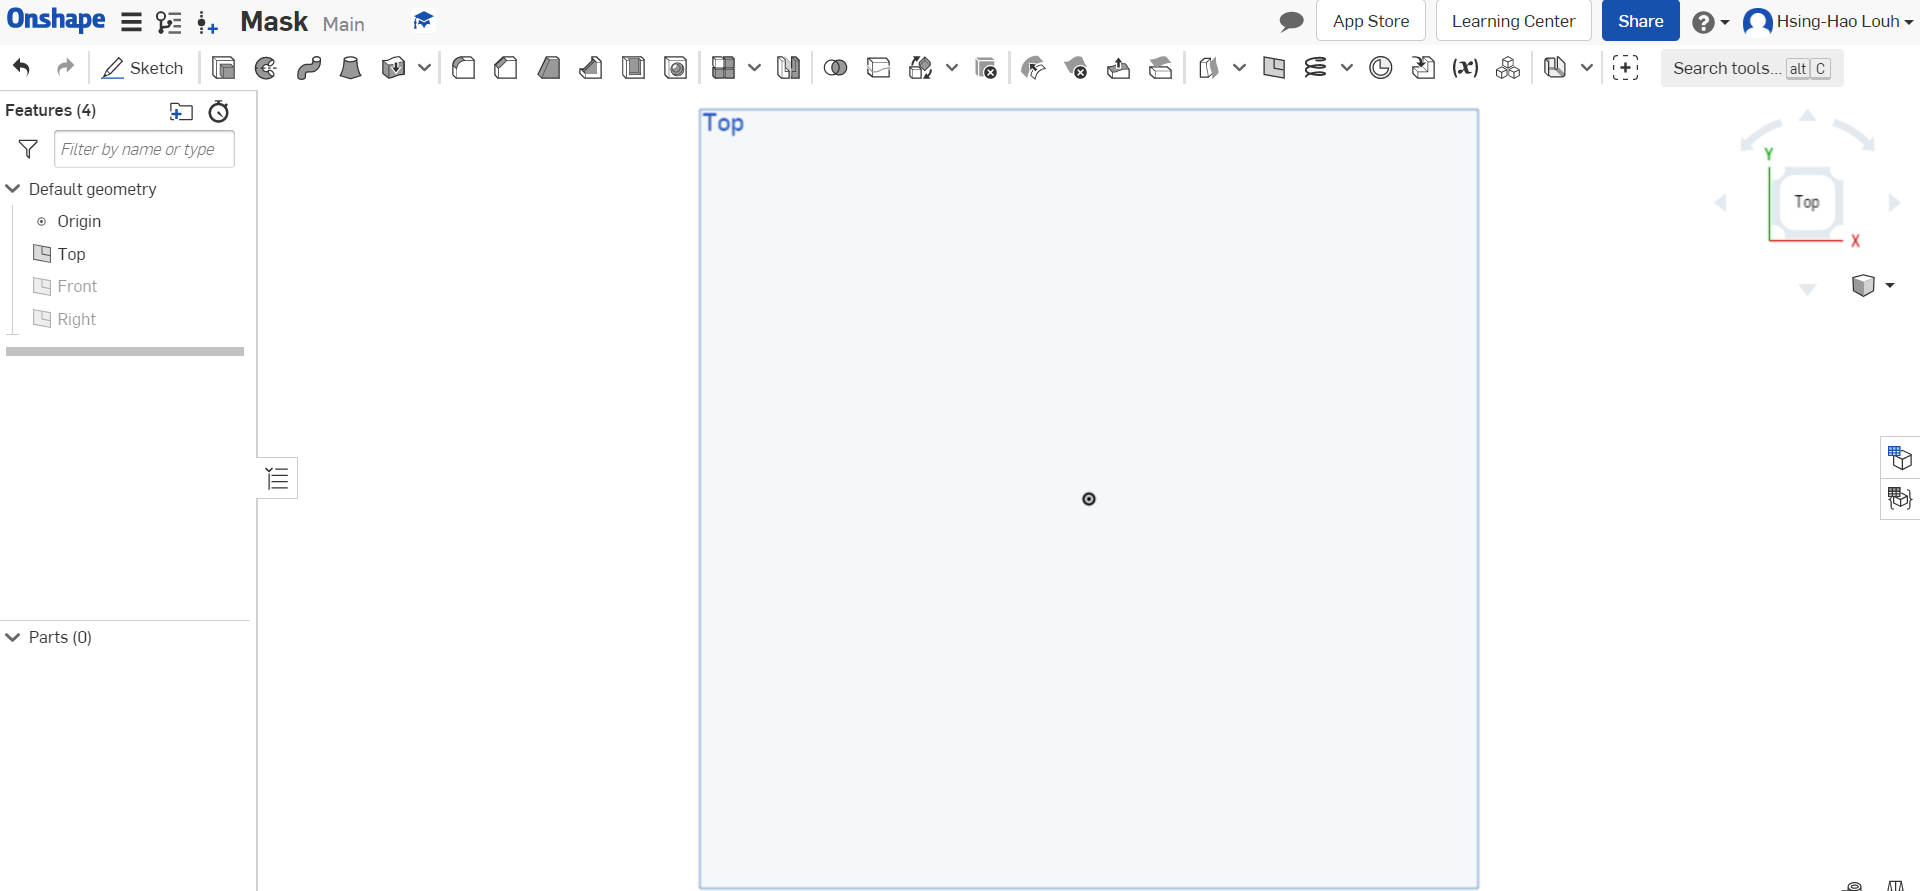
\includegraphics[width=0.8\textwidth]{figures/image3.png}
\end{figure}
\item To put our sketch on the {\bf Top} plane, click on $\vcenter{\hbox{
\includegraphics{figures/image4.png}}}$ in the top left and select the {\bf Top} plane.
\item To draw a {\bf circle}, select $\vcenter{\hbox{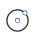
\includegraphics{figures/image5.png}}}$ for the mask. Left click on the origin and drag out some distance away and left click again. We will change the dimensions next.

\newpage
\item On the toolbar, click the {\bf dimension} button $\vcenter{\hbox{
\includegraphics{figures/image6.png}}}$ and left click anywhere on the circumference of the circle and left click again in the inside of the circle. Set the diameter to be {\bf 50mm}. This tool will help you dimension your drawings. Your screen should look like this:
\begin{figure}[ht!]
\centering
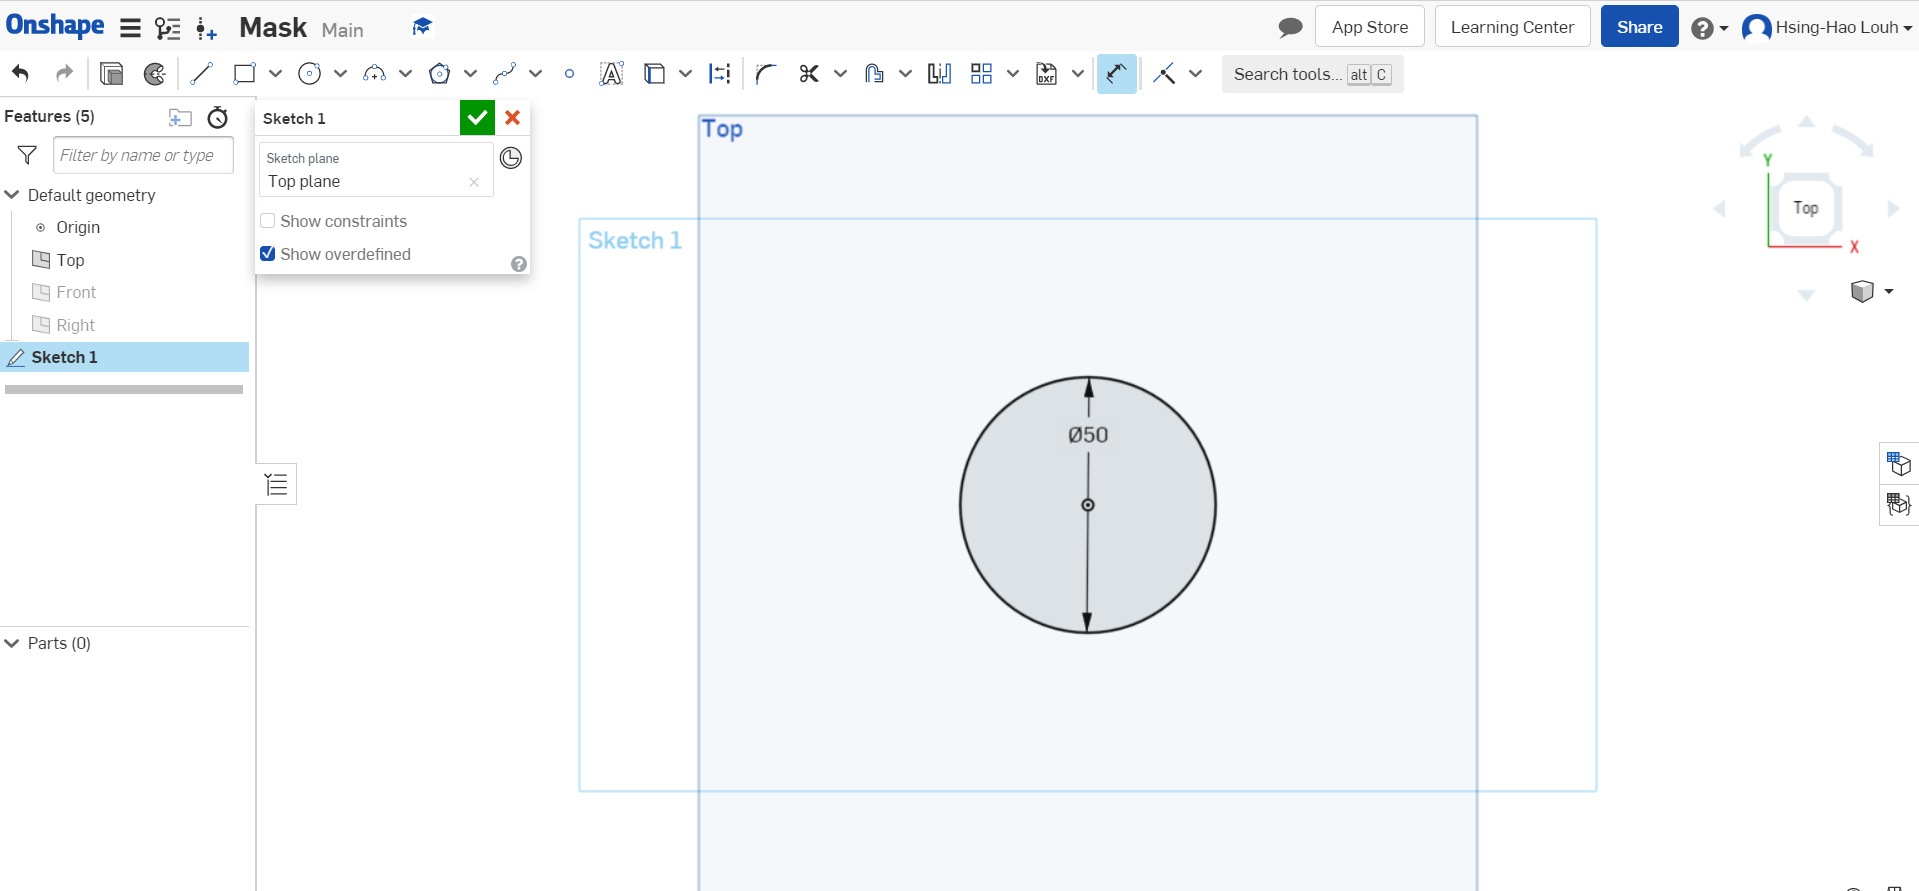
\includegraphics[width=0.8\textwidth]{figures/image7.png}
\end{figure}
\item On the top left click {\bf extrude} $\vcenter{\hbox{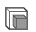
\includegraphics{figures/image8.png}}}$. If the circle is not already highlighted, click on it. Set the depth to be {\bf -5mm} and click the green checkmark $\vcenter{\hbox{
\includegraphics{figures/image9.png}}}$.
\item Now we will create a new sketch for a square where your designs will go in. Click {\bf sketch} $\vcenter{\hbox{
\includegraphics{figures/image4.png}}}$, select the top plane, and click on the little arrow to the right of the rectangle in the toolbar and select {\bf Center point} rectangle $\vcenter{\hbox{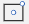
\includegraphics{figures/image11.png}}}$. Like the circle, click on the origin and drag out to anywhere inside the circle. Use the dimension tool $\vcenter{\hbox{
\includegraphics{figures/image6.png}}}$ to set the length of the sides to create a {\bf 34mm x 34mm} square. Your figure should now look as shown below. Keep all your designs within this square. Click the green checkmark $\vcenter{\hbox{
\includegraphics{figures/image9.png}}}$.
\begin{figure}[ht!]
\centering
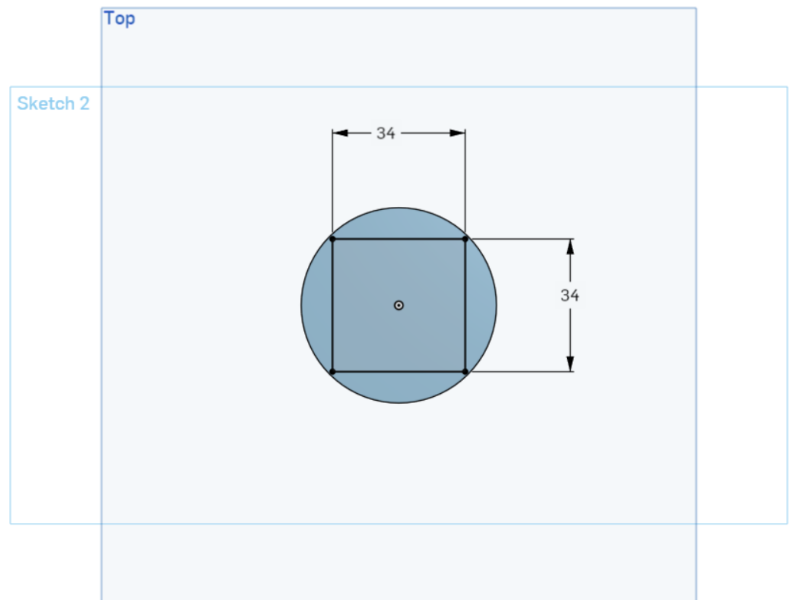
\includegraphics[width=0.5 \textwidth]{figures/image10.png}
\end{figure}
\end{enumerate}

\section{Adding your initials}
\begin{enumerate}
\setcounter{enumi}{9}
\item To add your initials, click {\bf sketch} $\vcenter{\hbox{
\includegraphics{figures/image14.png}}}$ and select the {\bf Face of your mask}. Click on the {\bf text} button $\vcenter{\hbox{
\includegraphics{figures/image15.png}}}$ on the toolbar. And click on the top half of the square to temporarily create the area your letters will go in. This can be moved later. Type your initials and select {\bf Arimo} for the font. To center your initials, click on the little arrow to the right of the {\bf Coincident} button $\vcenter{\hbox{
\includegraphics{figures/image16.png}}}$ and select {\bf vertical} $\vcenter{\hbox{
\includegraphics{figures/image17.png}}}$. Click on the midpoint of the bottom line of text box and then click on the origin and your initials should be centered. Click on vertical again to deselect this feature.
\item To engrave your initials, click on {\bf extrude} $\vcenter{\hbox{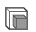
\includegraphics{figures/image8.png}}}$ and select the text. Select {\bf Remove} and set the depth to {\bf 2.5mm}. Your mask should look like the image below:
\begin{figure}[ht!]
\centering
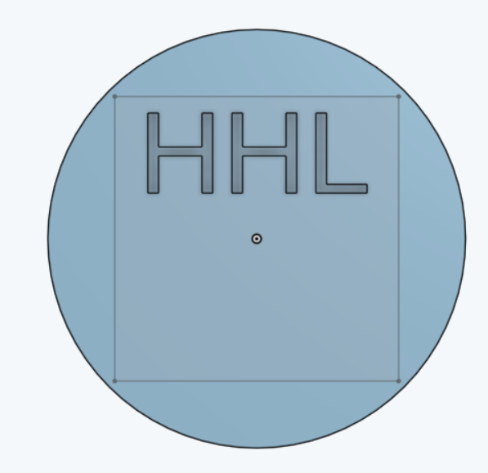
\includegraphics[width=0.5 \textwidth]{figures/image12.png}
\end{figure}
\end{enumerate}

\newpage
\section{Adding your design}
\begin{enumerate}
\setcounter{enumi}{11}
\item Create new sketches to create new designs and engrave them onto your mask. Be sure to select the face of mask when you create a new sketch. Play with the various features on the toolbar to help you create your design and use the {\bf dimension} tool $\vcenter{\hbox{
\includegraphics{figures/image6.png}}}$ to size your design. Make sure to keep your designs within the square.
\item Engrave your final design into your mask by selecting the design (you can click and drag to highlight your entire design or click on individual components) and follow the instructions on step 11. {\bf Only engraved parts will appear on the mask.} This means lines will not appear on the mask. The design below was created with only the {\bf Line} $\vcenter{\hbox{
\includegraphics{figures/image20.png}}}$  and {\bf dimension} $\vcenter{\hbox{
\includegraphics{figures/image19.png}}}$ features!
\begin{figure}[ht!]
\centering
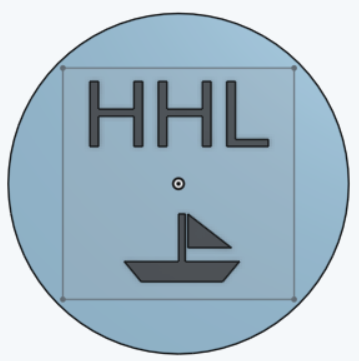
\includegraphics[width=0.5 \textwidth]{figures/image18.png}
\end{figure}
\item Highlight your engraved design by clicking and dragging. Right click on the highlighted area and select {\bf Add appearance to $\_$ faces} at the very bottom (the number in $\_$ depends on your sketch). Select black and click on the green checkmark $\vcenter{\hbox{
\includegraphics{figures/image9.png}}}$. 
\end{enumerate}
\newpage

\section{Sharing and Printing}
\begin{enumerate}
\setcounter{enumi}{14}
\item On the left panel, right click on {\bf Sketch 2} (the square should be highlighted) and click {\bf Edit}. Click {\bf extrude} $\vcenter{\hbox{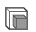
\includegraphics{figures/image8.png}}}$. Individually select each edge of the square and set the parameters as seenbelow. Note {\bf Surface} is selected, not Solid, and the depth is {\bf-2.5mm} not 2.5mm. Click on the green checkmark.
\begin{figure}[ht!]
\centering
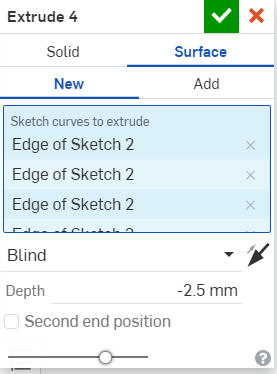
\includegraphics[width=0.5 \textwidth]{figures/image13.png}
\end{figure}
\item On the left panel, move your mouse over Sketch 2, and click on the eye $\vcenter{\hbox{
\includegraphics{figures/eye.png}}}$ to hide the sketch. Do the same for the origin.
\newpage
\item Save a PNG of your design by clicking on the three lines $\vcenter{\hbox{
\includegraphics{figures/image2.png}}}$  on the top left and selecting {\bf Print}. Set the paper to {\bf Letter} and {\bf Portrait}. A dotted area should appear on your screen to designate what are will be downloaded. Try to make the mask as big as possible without touching the dotted area, as shown on the image below. Click {\bf download image} and email it to your TA and the head TA Jerry Louh (\href{hl295@duke.edu}{hl295@duke.edu}). Include in your email your TA and lab section.
\begin{figure}[ht!]
\centering
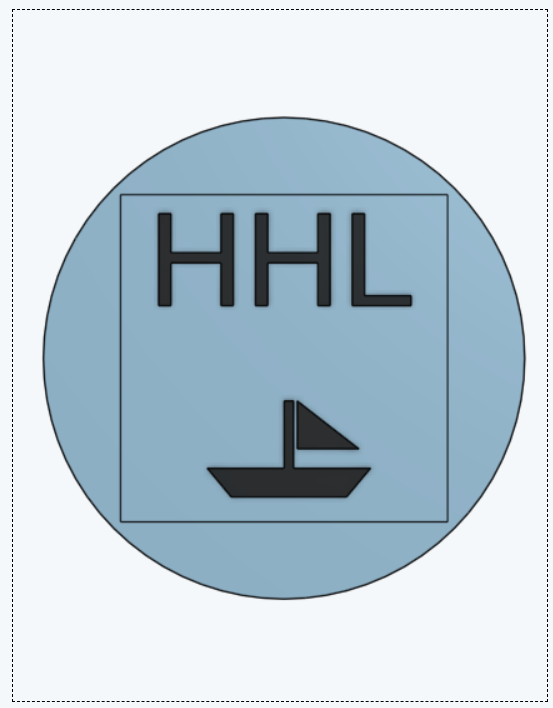
\includegraphics[width=0.5 \textwidth]{figures/final.png}
\end{figure}
\item After your TA approves your design, share your design with Jerry using $\vcenter{\hbox{
\includegraphics{figures/image22.png}}}$
\item Congratulations, you have designed a mask!
\end{enumerate}
\end{document}
